\documentclass{article}
\usepackage{hw_style}
\usepackage{enumerate}
\usepackage{graphicx}
\usepackage{verbatim}

% Homework Specific Information
\newcommand{\hmwkTitle}{Homework \#1}
\newcommand{\hmwkDueDate}{Friday Sept. 30th}
\newcommand{\hmwkAuthorName}{Kurt Rudolph}%Name:
\newcommand{\hmwkNetID}{rudolph9}%your netid
\newcommand{\hmwkNotes}{}%I worked with...

\newcommand{\hmwkSubTitle}{}
\newcommand{\hmwkClass}{CS 412}
\newcommand{\hmwkClassTime}{Wed, Fri 3:30PM - 4:45PM}
\newcommand{\hmwkClassInstructor}{Jiawei Han}

\begin{document}
\begin{spacing}{1.1}
\maketitle
%=============================Problem1=========================%
\newpage
\begin{homeworkProblem}
	We model the users in a social network as a data cube. Suppose each user has 10 dimensions of information, such as age, gender, city and income. Assume a base cuboid of 10 dimensions contains three base cells: (1) ($b1, b2, a3, a4, a5, \dots, a9, a10):count=10, (2) (b1, a2, b3, a4, a5, \dots, a9, a10):count=20$, and $(3) (a1, b2, b3, a4, a5, \dots, a9, a10$):count=50, where $a_i != b_i, a_i!=a_j$, etc. The count measure of the cube means the number of users who satisfy such information.
	
	\begin{enumerate}[(1)]
		\item How many nonempty cuboids will a full data cube contain?
			\begin{homeworkSection}{Solution}

			\end{homeworkSection}
		\item How many nonempty aggregate (i.e., non-base) cells will a full cube contain?
			\begin{homeworkSection}{Solution}

			\end{homeworkSection}
		\item How many nonempty aggregate cells will an iceberg cube contain if the condition of the iceberg cube is "count >= 70"?
			\begin{homeworkSection}{Solution}
				
			\end{homeworkSection}
		\item How many closed cells are in the full cube? 
			\begin{homeworkSection}{Solution}
				
			\end{homeworkSection}
	\end{enumerate}
\end{homeworkProblem}
%=============================Problem2==========================%	
\begin{homeworkProblem}
	Given the following base cuboid with count as the measure.\\
	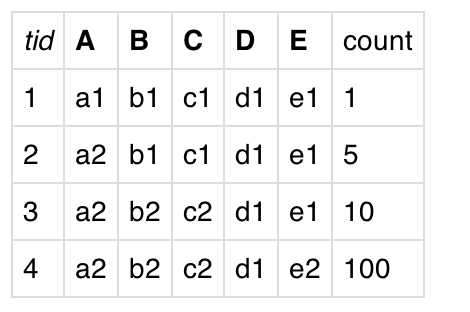
\includegraphics[width=\linewidth /2]{prob2.png}
	\begin{enumerate}[(1)]
		\item Briefly outline the major steps to compute Shell-Fragment cube (refer to VLDB04 paper �High-Dimensional OLAP: A Minimal Cubing Approach�), suppose we divide the 5 dimensions into 2 shell fragments: AB and CDE.
			\begin{homeworkSection}{Solution}

			\end{homeworkSection}
		\item Briefly describe how to compute subcube query (a2,b2,,,? : count()) 
			\begin{homeworkSection}{Solution}

			\end{homeworkSection}
	\end{enumerate}
\end{homeworkProblem}
%=============================Problem3==========================%	
\begin{homeworkProblem}
	Given a database of five transactions ($min_support = 2$):
	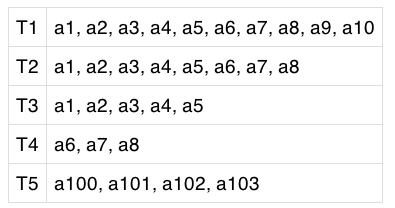
\includegraphics[width=\linewidth /2]{prob3.png}
	\begin{enumerate}[(1)]
		\item How many frequent patterns?
			\begin{homeworkSection}{Solution}

			\end{homeworkSection}
		\item What is the set of frequent closed patterns (list both pattern and support)? 			\begin{homeworkSection}{Solution}

			\end{homeworkSection}
		\item What is the set of frequent max-patterns (list both pattern and support)? 
			\begin{homeworkSection}{Solution}

			\end{homeworkSection}
		\item Show an example association rule that matches $(a1, a2, a3, a4, itemX) -> (itemY) [min_support = 2, min_confidence=70\%]$
			\begin{homeworkSection}{Solution}
  
			\end{homeworkSection}
		\item For association rule a1->a6, compute the following measures: confidence, lift, kulc.
			\begin{homeworkSection}{Solution}
  
			\end{homeworkSection}
		\item Among the above three measures, which ones are null-invariant? 
			\begin{homeworkSection}{Solution}
  
			\end{homeworkSection}
	\end{enumerate}
\end{homeworkProblem}
%=============================Problem4==========================%	
\begin{homeworkProblem}
	Given a database of four transactions $(min_support = 2)$:
	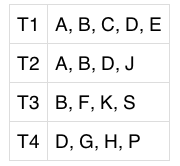
\includegraphics[width=\linewidth /2]{prob4.png}
	\begin{enumerate}[(1)]
		\item Show the major steps to find the frequent patterns using Apriori.
			\begin{homeworkSection}{Solution}

			\end{homeworkSection}
		\item Show the major steps to find the frequent patterns using FP-Growth (no need to draw the trees).
			\begin{homeworkSection}{Solution}

			\end{homeworkSection}
		\item Compare the three algorithms: Apriori, FP-growth and ECLAT, by concisely discussing the major differences.  
			\begin{homeworkSection}{Solution}

			\end{homeworkSection}
	\end{enumerate}
\end{homeworkProblem}

	
\end{spacing}
\end{document}

\begin{comment}%==========================================================
%=============================Problemi==========================%	
\begin{homeworkProblem}
	
	\begin{homeworkSection}{Solution}
		
	\end{homeworkSection}
\end{homeworkProblem}
%=============================Problemi==========================%	
\begin{homeworkProblem}
	
	\begin{enumerate}[(a)]
		\item 
			\begin{homeworkSection}{Solution}
		
			\end{homeworkSection}
	\end{enumerate}
\end{homeworkProblem}
%=============================Problemi==========================%	
\begin{homeworkProblem}
	{\bf }	
	\begin{homeworkSection}{Solution}
		
	\end{homeworkSection}
\end{homeworkProblem}
%=============================Problemi==========================%	
\newpage
\begin{homeworkProblem}
	{\bf  }	
	\begin{enumerate}[(a)]
		\item 
			\begin{homeworkSection}{Solution}
		
			\end{homeworkSection}
	\end{enumerate}
\end{homeworkProblem}
%=============================Problemi=========================%
\newpage
\begin{homeworkProblem}
	
	\begin{homeworkSection}{Solution}
		
	\end{homeworkSection}
\end{homeworkProblem}

\end{comment}%=========================================================
















